\chapter{Etat de l'art}
\authors{
  \authorinfo{Marc}{de la Motte Rouge} \\
}

Pour orienter notre projet, nous avons d'abord observ� les diff�rentes solution d�ja mises en oeuvre dans des projets similaires. Nous avons �tudi� les possibilit�s propos�es pour chaque partie ainsi que l'inter�t qu'elles pr�sentaient pour nous par rapport � l'objectif p�dagogique du projet.

\section{L'appareil}
La majorit� des projets d�ja cr��s, utilisent des airbus A320 ou des Boeing 737. L'�lectronique de ces appareils est "relativement simple" � mettre en oeuvre car ce sont des appareils de "petite taille".  Quelque projet utilisent des appareils plus important. Ils sont souvent destin�s � la formation du personel naviguant. 

\section{Les bus de donn�es}

\section{La partie commande}

\section{Affichage}
Lors de nos recherches effectu�es sur le monde ext�rieur, nous avons trouver un moyen pour partager l'image provenant de FSUIPC sur plusieurs �crans. Un module, le TripleHead2Go, permet d'effectuer cette op�ration. Les diff�rents �crans sont connect�s au module via des c�bles VGA. Ce syst�me est ainsi vu par l'unit� centrale come �tant un �cran ultra large (c'est � dire 3840x1024). Le sch�ma suivant donne une repr�sentation de l'agencement du module.

\begin{figure}[htpb]
  \centering
  \fbox{
    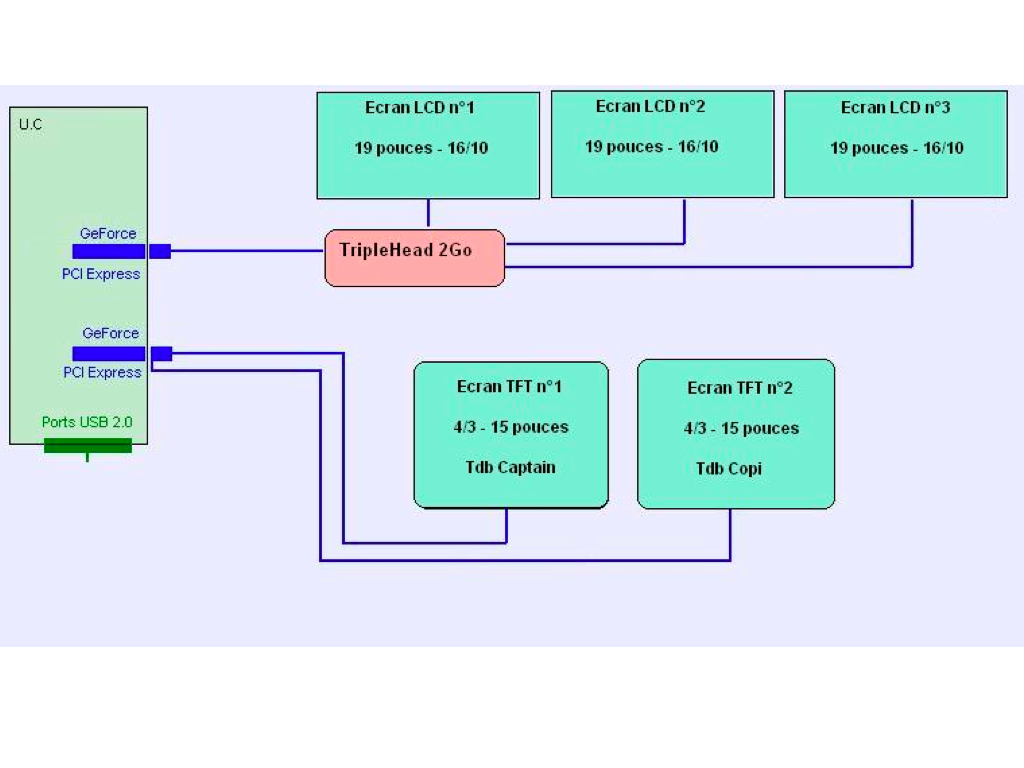
\includegraphics[scale=0.3]{images/schema-diviseur-ecran}
  }
  \caption{Sch�ma globale de la connexion des �crans avec le module TripleHead2Go}
  \label{fig:schema-diviseur-ecran}
\end{figure}
